\documentclass{ctexart}

%%%% Chinese support
%

%%%% Page geometry
\usepackage[
    a4paper,
    total={210mm,297mm},
    left=20mm,
    right=20mm,
    top=20mm,
    bottom=20mm,
  ]{geometry}            %

%%%% Math
\usepackage{amsmath}     %
\usepackage{siunitx}     % SI unit support
\usepackage{bm}             % Bold and Italic math font for vector
\usepackage{commath} % differential operator

%%%% Caption
\usepackage{caption}
\captionsetup{belowskip=8pt,aboveskip=4pt}


%%%% Graph processing
\usepackage{graphicx}    % graph inclusion

%%%% Table processing
\usepackage{tabularx}
\usepackage{booktabs}    %
\usepackage{csvsimple}   % CSV table processing
\usepackage{multirow}    % multirow in table

%%%% Hyper reference
\usepackage[
    bookmarksnumbered=true,
    colorlinks=true,
    allcolors=blue,
  ]{hyperref}             %

%%%% Bibliography
\usepackage[
    backend=biber,
    style=numeric,
    citestyle=ieee,
    bibencoding=utf8,
  ]{biblatex}             %
\addbibresource{compact_debris_cfd.bib}

\usepackage{textcomp}

\title{龙卷风风场中块状飞射物的飞行特性:计算流体力学模拟}
\author{王勇}

\begin{document}
\maketitle
\begin{abstract}
本文主要通过计算流体力学方法模拟龙卷风风场中块状飞射物的飞行特性。
首先利用ANSYS Fluent 计算流体力学软件模拟龙卷风风场,并与多普勒雷达实测龙卷风风场对比,以检验模拟结果的正确性。
然后介绍ANSYS Fluent的离散相模型,以模拟在龙卷风风场中块状飞射物的运动。
最后通过一个算例比较本文的模拟方法与解析方法的结果。
\end{abstract}

\section{龙卷风的数值模拟} \label{sec:tornado_simulation}
实际情况中龙卷风的风场结构十分复杂,不仅有着单涡和多涡等多种形式,还具有一定的平移速度。
出于简化影响因素的考虑,本文仅模拟单涡形式的龙卷风,且假定龙卷风为定常风场。
并且部考虑龙卷风的平移运动,忽略地面粗糙度的影响。

\subsection{龙卷风发生装置}
本文模拟龙卷风的物理模型,是基于东京理工大学Matsui等人\cite{matsui2009}设计的实验室龙卷风模拟装置(见图\ref{fig:matsui_tornado_generator})。
为了模拟1998年5月30日多普勒雷达测得的美国南达科他州地区实际发生的一个龙卷风,本文采用全尺寸模型,调整了模型中各部分的尺寸参数,最后确定了龙卷风数值模型的物理发生装置\cite{tang2013}。
该发生装置的具体形式如图\ref{fig:tornado_generator}所示,模型各部分尺寸及参数设置见表\ref{tab:tornado_generator_parameters}。

\begin{figure}[h!]
\centering
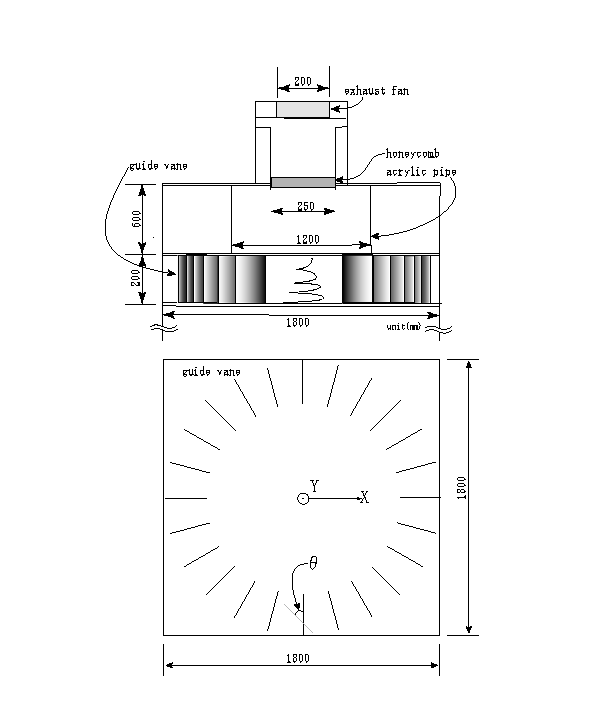
\includegraphics[width=0.8\textwidth]{./fig/matsui_tornado_generator}
\caption{龙卷风实验装置(\cite{matsui2009})}
\label{fig:matsui_tornado_generator}
\end{figure}

\begin{figure}[h!]
\centering
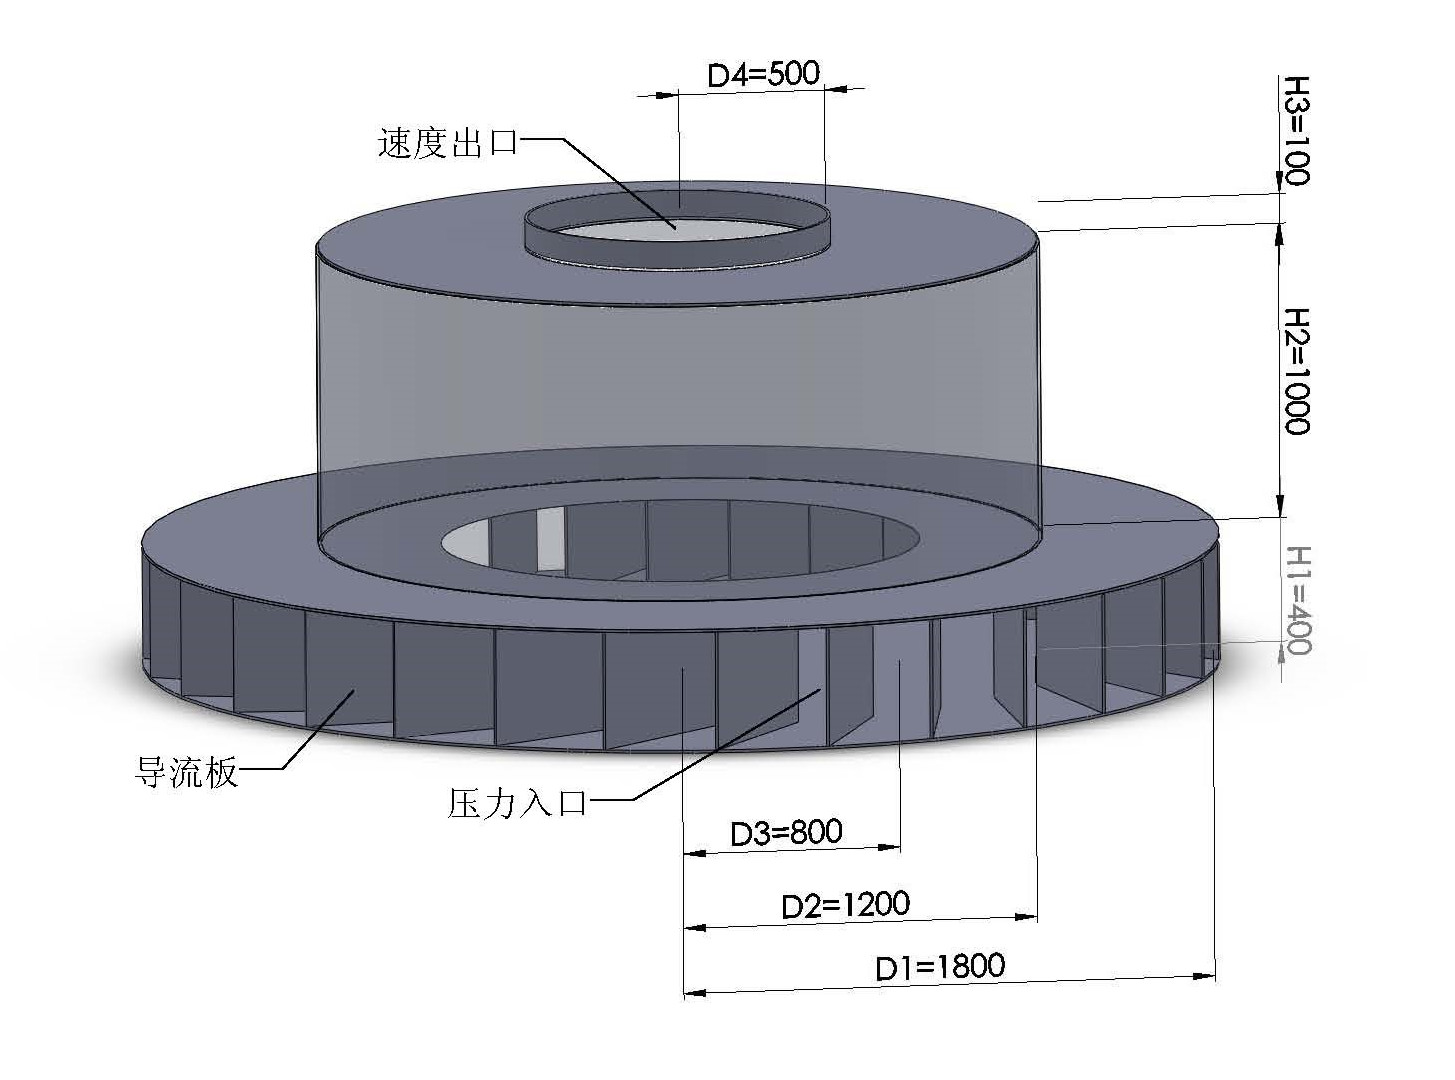
\includegraphics[width=0.9\textwidth]{./fig/tornado_generator}
\caption{龙卷风数值模拟模型}
\label{fig:tornado_generator}
\end{figure}

\begin{table}[h!]
\caption{龙卷风发生装置尺寸参数}
\label{tab:tornado_generator_parameters}
\centering
\begin{tabular*}{\textwidth}{c @{\extracolsep{\fill}} c c c c c c c}
    \toprule
   导流板角度$\theta (\SI{}{\degree})$ & $D1(\SI{}{m})$ & $D2(\SI{}{m})$ & $D3(\SI{}{m})$ & $H1(\SI{}{m})$ &  $H2(\SI{}{m})$ &  $H3(\SI{}{m})$ & 出口速度$(\SI{}{m/s})$ \\
   \midrule
   30 & 1800 & 1200 & 800 & 400 & 1000 & 100 & 52.5 \\
   \bottomrule
\end{tabular*}
\end{table}


\subsection{龙卷风的数值模型}\label{sec:tornado_cfd}
采用ANSYS Fluent\textregistered 计算流体力学软件对龙卷风进行数值模拟。

\subsubsection{计算区域网格的划分}
由于模型比较复杂,流域网格采用适应性良好的四面体非结构网格,如图\ref{fig:mesh}所示。

\begin{figure}[h!]
\centering
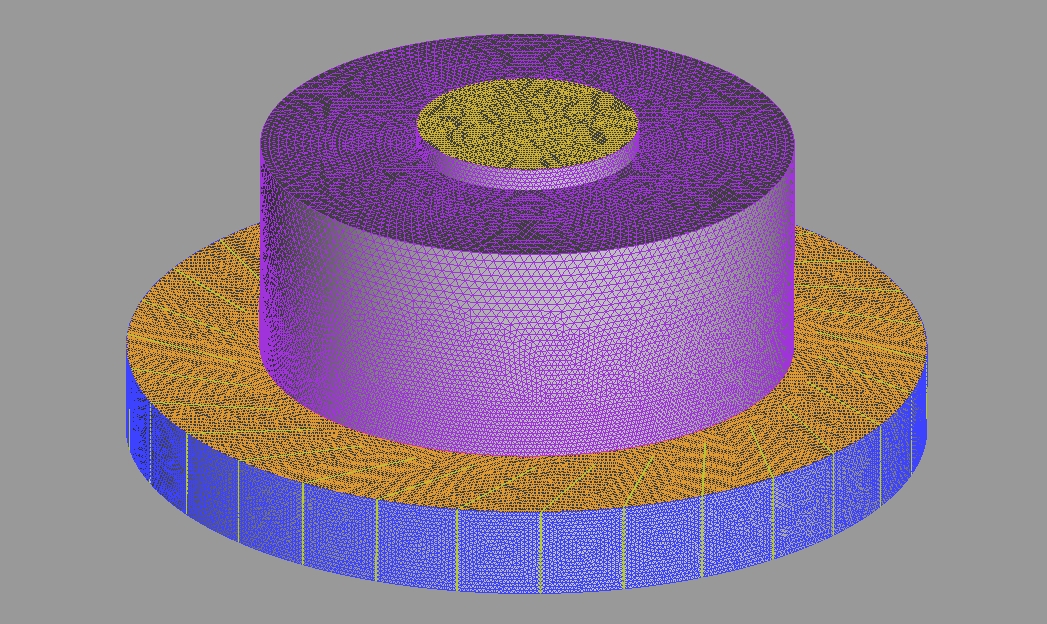
\includegraphics[width=\textwidth]{./fig/mesh}
\caption{龙卷风数值模拟的网格划分示意图}
\label{fig:mesh}
\end{figure}

由于主要关心的是近地面附近龙卷风对结构的作用,故对近地面流域处的网格进行了细分。
通过加密网格的方式,来探讨网格对计算结果的影响。
不断加密网格直到监测平面处的最大切向速度和最大切向速度所在半径的位置前后两次计算结果相差小于$5 \%$。
最后根据计算机的能力及计算结果的有效性,确定目前所采用的网格形式。

\subsubsection{湍流模型及求解设定}
本文采用三维定常计算方法,获得了龙卷风风场中各变量的时均信息。
湍流模型选取应用较广泛的RNG $k-\varepsilon$模型,近壁面采用非平衡面函数(Non-Equilibrium Wall Functions)。
离散格式采用精度较高的二阶迎风格式,离散后控制方程的求解采用压力修正的分离式解法——SIMPLEC算法。

\subsubsection{边界条件的选取}
底部入口采用压力入口(pressure-inlet),入口处的压力值与标准大气压相等;
顶部出口采用速度出口(velocity-outlet),速度方向与出口边界垂直,速度大小为\SI{52.5}{m/s};
地面、导流板以及周围筒体均采用无滑移壁面边界条件(wall)。


\subsection{数值模拟结果及正确性验证}\label{sec:cfd_verification}
\subsubsection{数值模拟龙卷风的特征参数}
经软件计算,得到\SI{20}{m}高度处数值模拟龙卷风的重要特征参数如表\ref{tab:cfd_tornado_parameters}所示。
\begin{table}[h!]
\caption{数值模拟龙卷风\SI{20}{m}高度处的特征参数}
\label{tab:cfd_tornado_parameters}
\centering
\begin{tabular*}{\textwidth}{c @{\extracolsep{\fill}} c c c}
    \toprule
   龙卷风等级 & 最大旋转风速$V_{\mathrm{R}} (\SI{}{m/s})$ & 最大旋转风速半径$R(\SI{}{m})$ & 压力降$\Delta P (\SI{}{Pa})$ \\
   \midrule
   EF4 & 82.3 & 117.6 & -9841.8\\
   \bottomrule
\end{tabular*}
\end{table}

数值模拟得到的最大旋转风速为\SI{82.3}{m/s},最大旋转风速半径为\SI{117.6}{m};
而多普勒雷达测得\SI{20}{m}高度处的最大旋转风速为\SI{81.6}{m/s},最大旋转风速半径为\SI{118.6}{m}.
可见,数值模拟可较好地模拟多普勒雷达实测龙卷风的最大切向速度和最大切向速度半径。
由于本文不考虑龙卷风气压降对块状飞射物飞行的影响,故不再验证数值龙卷风模型的气压降。

\subsubsection{切向速度的分布特征}
图\ref{fig:Vr}为\SI{20}{m}高度处龙卷风的切向速度随其半径的变化曲线图,包括:
\SI{20}{m}高度处数值龙卷风模拟结果,Rankine涡模型结果及美国南达科他州Spencer地区实际发生龙卷风\SI{20}{m}高度处的多普勒雷达实测结果。

\begin{figure}
\centering
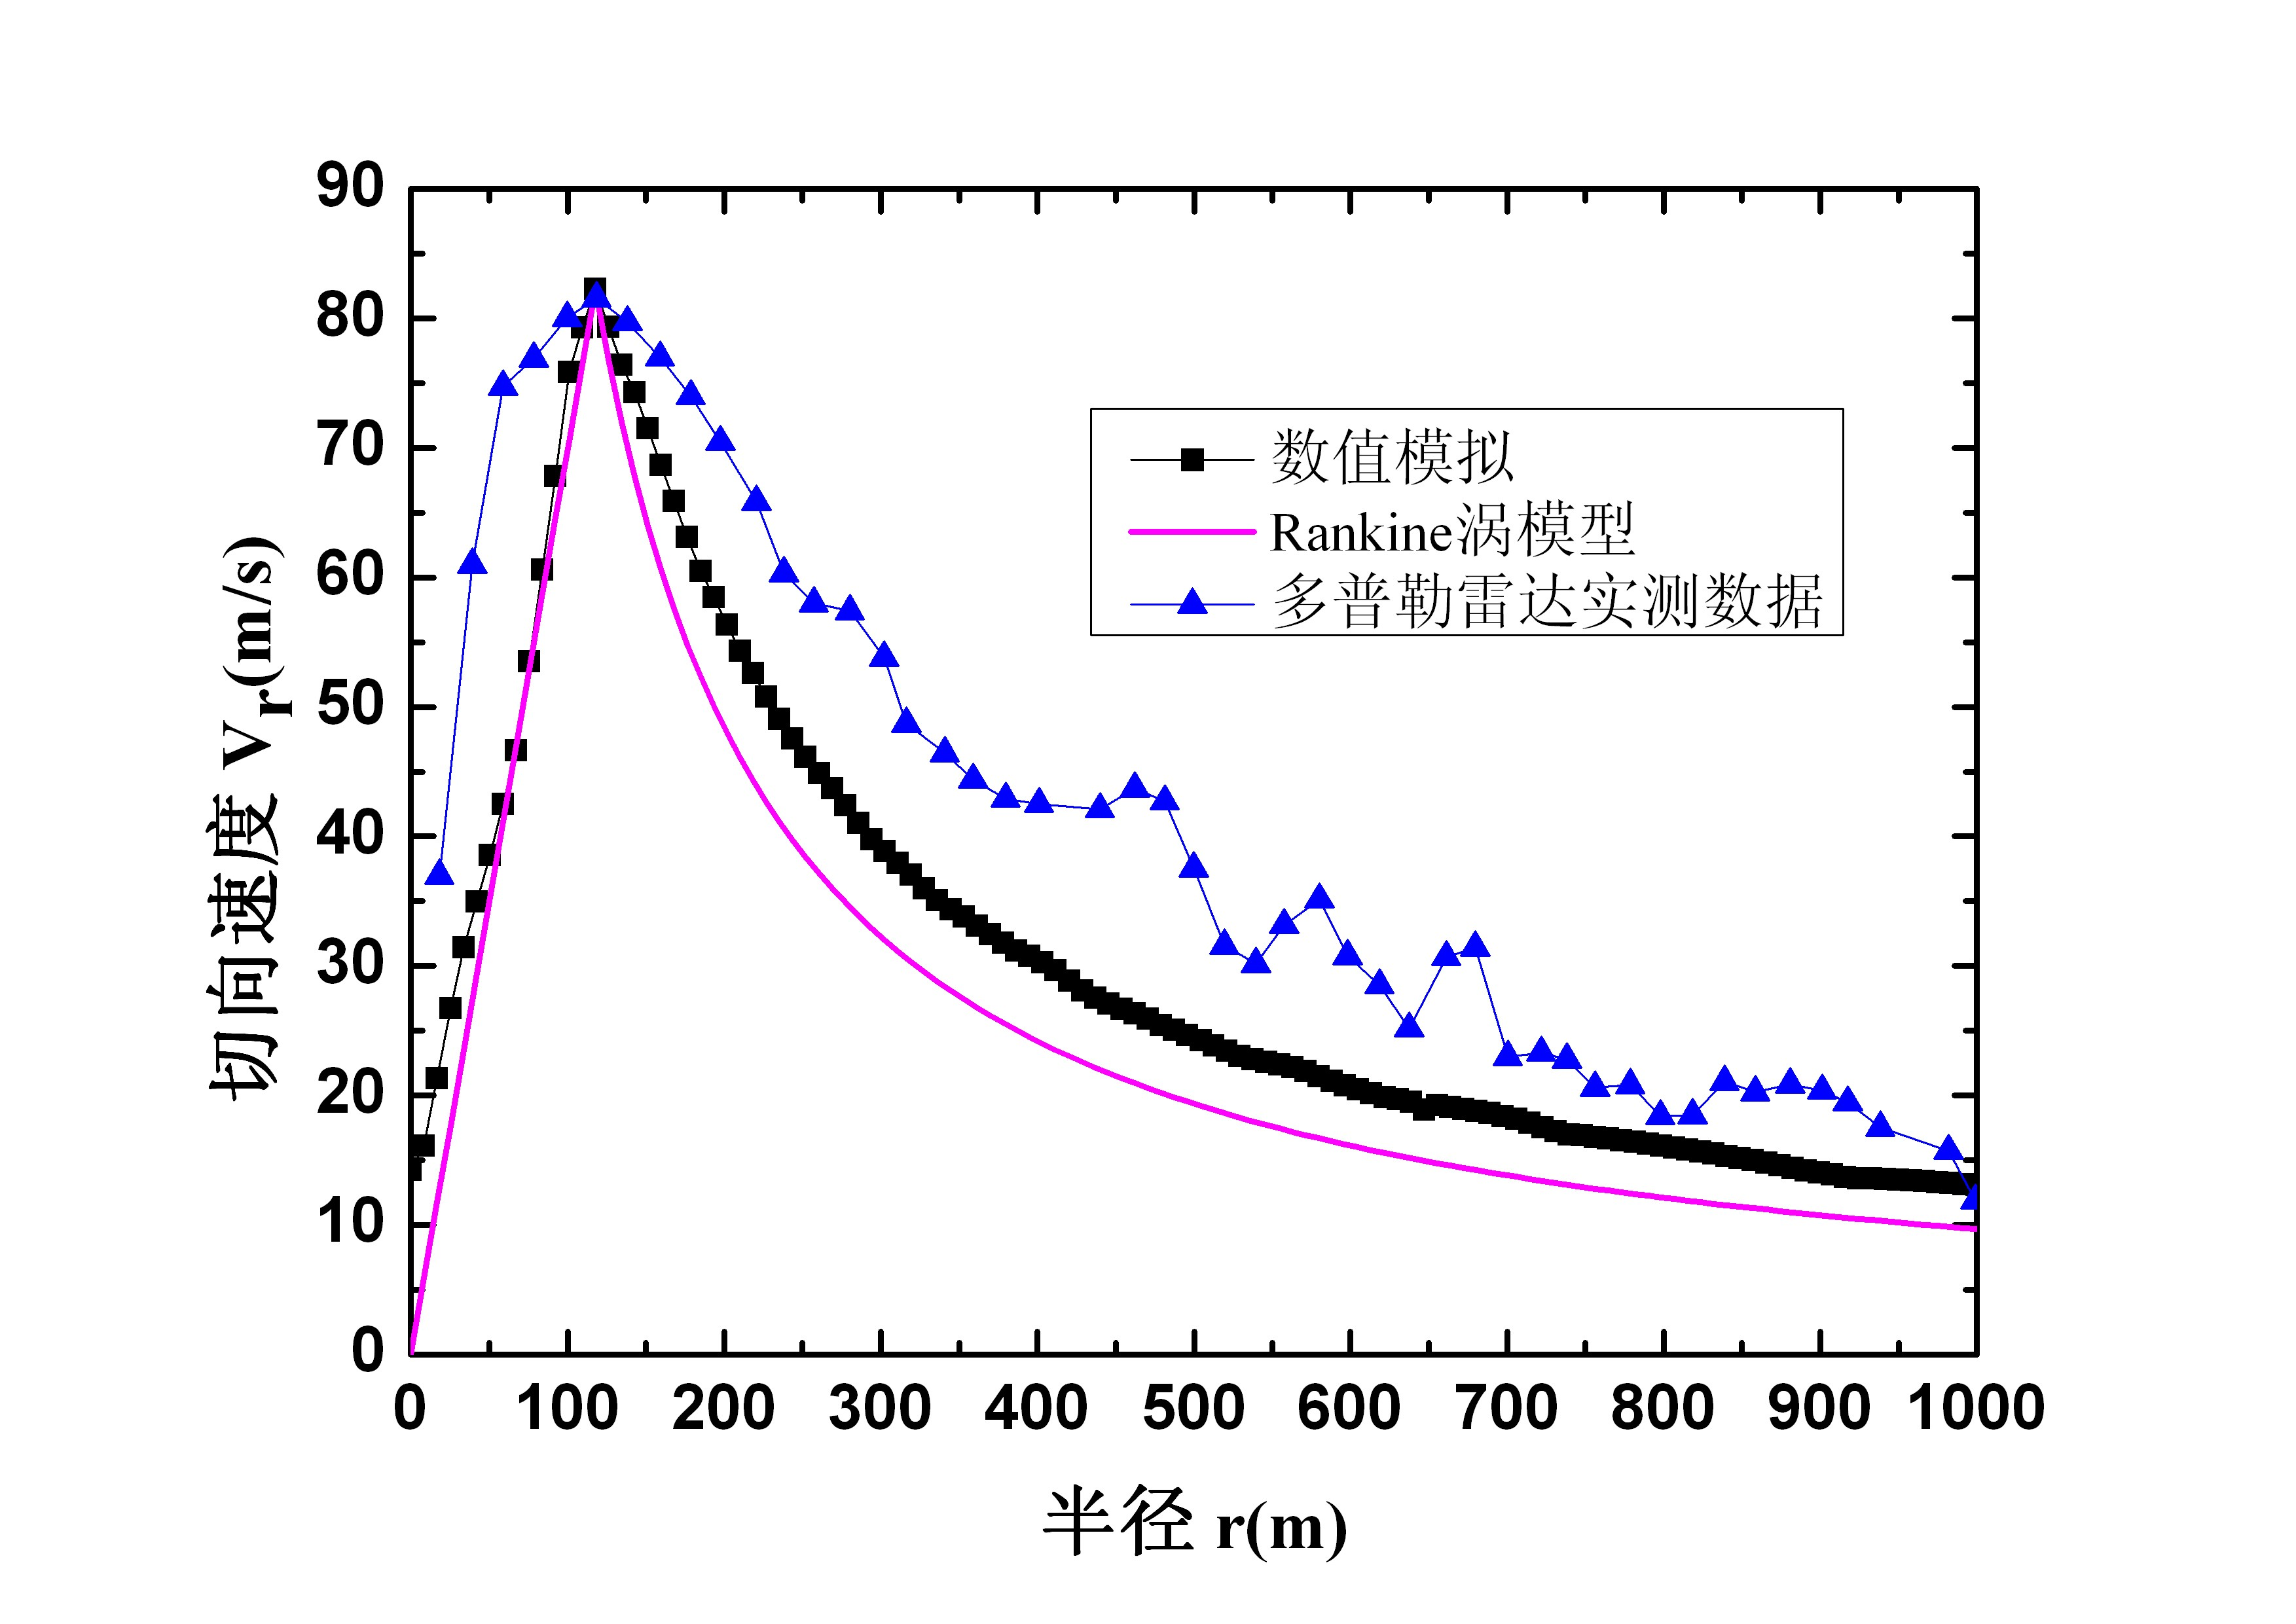
\includegraphics[width=0.8\textwidth]{./fig/Vr}
\caption{\SI{20}{m}高度处龙卷风切向速度随半径变化示意图}
\label{fig:Vr}
\end{figure}


从图中可以看出,Rankine涡模型和数值模拟的结果都较好地模拟了美国南达科他州Spencer地区实际发生的龙卷风,能反映出龙卷风切向速度随其半径的变化规律。
实际情况中,龙卷风是非定常,雷达观测到的数据是通过时间平均得到的。
本文数值模拟方法假定龙卷风是定常的,利用固定的边界条件和初始条件模拟了定常的龙卷风涡结构,与实际的龙卷风略有不同。
并且本文数值模拟方法采用的是均匀沙粒状的地表面,与实际地面粗糙度可能并不一致,从而导致摩擦力的影响有所不同,而Rankine涡模型甚至没有考虑摩擦力的影响。
由于这些偏差的存在,使得数值模拟结果不可能完全与Rankine涡模型以及雷达观测的数据一致。


\section{离散相模型的基本理论}
利用ANSYS Fluent\textregistered 中的离散相模型求解飞射物在龙卷风风场中的飞行问题\cite{fluent2011}。
其中流体相(空气)的详细信息通过在Euler坐标系中求解连续方程和Navier-Stokes方程获得,而飞射物当成离散的颗粒(离散相),各项信息通过在Langrange坐标系中计算颗粒在流体相(空气)中的运动得到。

\subsection{颗粒的运动分析}
在Lagrange坐标系中,根据牛顿第二定律,颗粒的运动微分方程为\cite{fluent2011}:
\begin{equation}\label{eqn:ode_particle}
\od{\bm{u}_p}{t} = \frac{\bm{u}-\bm{u}_p}{\tau_r} + \frac{\bm{g} \left( \rho_p - \rho \right)}{\rho_p} + \bm{F}
\end{equation}
其中,$\frac{\bm{g} \left( \rho_p - \rho \right)}{\rho_p}$是单位质量颗粒受到的有效重力(颗粒重力减去所受的浮力),$\frac{\bm{u}-\bm{u}_p}{\tau_r}$是单位质量颗粒受到的流体阻力,$\bm{F}$是除净重力和流体阻力外的颗粒单位质量受到的惯性力(本文忽略颗粒受到的该项作用力)。对于阻力项,有
\begin{equation}\label{eqn:tau_r}
\tau_r=\frac{\rho_d d_p^2}{18 \mu} \frac{24}{C_D \mathrm{Re}}
\end{equation}
其中,$\tau_r$为颗粒的释放时间,$\bm{u}$是离散相的风速,$\bm{u}_p$是颗粒速度,$\mu$是流体粘滞系数,$\rho$是流体密度,$\rho_p$是颗粒密度,$d_p$是颗粒直径。$\mathrm{Re}$是相对雷诺数,定义为:
\begin{equation}
\mathrm{Re} \equiv \frac{\rho d_p\lvert \bm{u}_p-\bm{u} \rvert}{\mu}
\end{equation}

\subsection{阻力系数$C_D$}
光滑球状颗粒受到的阻力系数$C_D$可写成如下形式\cite{morsi1972}:
\begin{equation}
C_D = \alpha_1 + \frac{\alpha_2}{\mathrm{Re}} + \frac{\alpha_3}{\mathrm{Re}^2}
\end{equation}
式中$\alpha_1$,$\alpha_2$和$\alpha_3$是拟合光滑球体阻力系数的实验曲线的参数,与雷诺数所在的范围有关。

\subsection{离散相模型的边界条件}
当颗粒到达模型物理边界(如壁面、入口或出口)上时,ANSYS Fluent \textregistered 利用离散的边界条件来确定颗粒在边界上应该满足的条件。
ANSYS Fluent \textregistered 离散相模型中包含以下几种可选的边界条件。

\begin{description}
\item[reflect: ]
颗粒在此处发生反弹而产生动量变化,其变化量是通过反弹系数来确定,如图\ref{fig:bc}(a)所示。法向恢复系数确定了颗粒与壁面发生碰撞之后,在垂直于壁面方向的动量变化率,定义为:
\begin{equation}
e_n = \frac{v_{2,n}}{v_{1,n}}
\end{equation}
式中,$v_n$是垂直壁面的法向速度分量,下标1、2分别表示碰撞前后。同理,切向恢复系数可以确定颗粒与壁面碰撞之后,在壁面切向方向的动量变化率。

\item[trap: ] 颗粒在此处终止了其轨迹的计算,并且轨迹的结果标记为trapped,如图\ref{fig:bc}(b)所示。

\item[escape: ] 颗粒在此处被标记为escaped,并终止了其轨迹的计算,如图\ref{fig:bc}(c)所示。

\end{description}

\begin{figure}
\centering
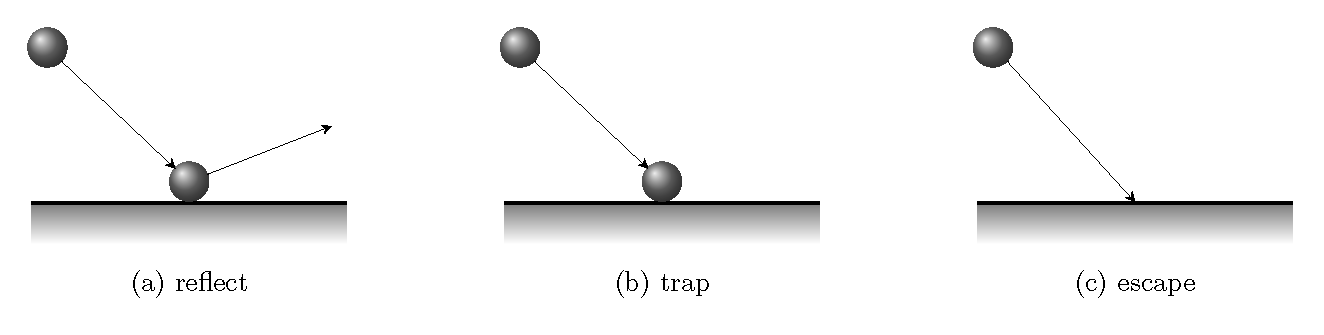
\includegraphics{./fig/bc}
\caption{离散相边界条件示意图}
\label{fig:bc}
\end{figure}

\subsection{离散相模型的求解过程}
ANSYS Fluent\textregistered 离散相模型中稳态问题的求解过程如图\ref{fig:dpm_flow}所示。
首先是求解连续相流场。
当连续相流场计算稳定后,通过定义离散相颗粒的初始位置、初始速度、尺寸大小等来创建离散相模型。
最后求解离散相,得到离散相模型中颗粒运动的各项信息。

\begin{figure}
\centering
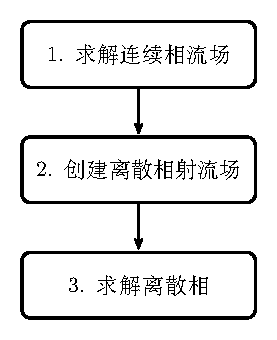
\includegraphics{./fig/dpm_flow}
\caption{ANSYS Fluent 离散相模型中稳态问题的求解过程示意图}
\label{fig:dpm_flow}
\end{figure}

离散相模型中的颗粒轨迹,是在离散的时间步长上逐步积分运算求解得到的,下面为数值求解方法的具体过程。
$x$轴方向上,颗粒的运动微分方程\eqref{eqn:ode_particle}可以写成如下形式:
\begin{equation}\label{eqn:ode_particle_i}
\od{u_{p}}{t} = \frac{1}{\tau_p}\left(u-u_{p}\right) +a_x
\end{equation}
式中,$\tau_p$为颗粒松弛时间,见式\eqref{eqn:tau_r},$a_x$包含除阻力外其他作用力所引起的加速度在$x$轴的分量。

ANSYS Fluent\textregistered 默认采用梯形差分格式对方程\eqref{eqn:ode_particle_i}进行离散求解。
假设其他作用力所产生的加速度$a_x$在离散时间步长$\Delta t$内为一常数,可以得到:
\begin{equation}
\frac{u_{p}^{n+1}-u_{p}^{n}}{\Delta t} = \frac{1}{\tau_p} \left( \bar{u}-\bar{u}_{p}\right) + a_x
\end{equation}
式中,$n$表示时间步,$\bar{u}$、$\bar{u_p}$分别为流体、颗粒在时间步$n$和$n+1$速度的平均值,计算公式为:
\begin{equation}
\begin{split}
\bar{u} = \frac{1}{2} \left(u^{n+1}+u^{n}\right) \\ 
\bar{u}_p = \frac{1}{2} \left(u_p^{n+1}+u_p^{n}\right) \\
u^{n+1} = u^{p} +\left( \bm{u}_P^n\cdot \nabla \bm{u}^n \right) \Delta t 
\end{split}
\end{equation}

因此,得到颗粒速度在第$n+1$时间步的值为:
\begin{equation}
u_{p}^{n+1}=\frac{u_{p}^{n}\left(   1- \frac{1}{2}\frac{\Delta t}{\tau_p} \right)+\frac{\Delta t}{\tau_p}\left[    u^n + \frac{1}{2} \left( \bm{u}_p^n\cdot \nabla \bm{u}^n \right) \Delta t    \right]+a_x \Delta t}{1+\frac{1}{2}\frac{\Delta t}{\tau_p}}
\end{equation}

而颗粒的轨迹方程可写成如下形式:
\begin{equation}\label{eqn:x}
\od{x_p}{t} = u_p
\end{equation}
采用隐性梯形差分格式,颗粒的新位置可通过对方程\eqref{eqn:x}梯度离散求解得到:
\begin{equation}
x_p^{n+1} = x_{p}^{n} + \frac{1}{2} \left( u_p^{n}+u_{p}^{n+1}\right) \Delta t 
\end{equation}

在已知的流场中,对于一个给定的时刻,求解颗粒运动平衡微分方程\eqref{eqn:ode_particle_i}和颗粒轨迹方程\eqref{eqn:x}就可以确定颗粒在流场中的速度与位置。

\section{算例}
选用表\ref{tab:cfd_tornado_parameters}中龙卷风的特征参数,即$V_{\mathrm{R}}=\SI{82.3}{m/s}$,$R = \SI{117.6}{m}$。飞射物为石质圆球,直径$d=\SI{8}{mm}$,密度为$\rho_m=\SI{2000}{kg/m^3}$,则$\ell =\frac{2}{3}d=\SI{5.33}{mm}$。

假设圆球释放位置据龙卷风涡旋中心的径向距离$r_0=\SI{300}{m}$,释放位置距地面高$z_0=\SI{20}{m}$。
分别按照如下情形进行计算:
\begin{description}
\item[Case 1: ] 采用《龙卷风风场中块状飞射物的飞行特性:解析方法》中考虑竖向速度对风阻力影响的小时间步积分法计算飞射物的运动过程。
\item[Case 2: ] 
利用ANSYS Fluent\textregistered 提供的UDF功能 将第\ref{sec:tornado_cfd}节的龙卷风风场初始化为Rankine涡模型,然后释放飞射物进行离散相的计算。
\item[Case 3: ] 
利用ANSYS Fluent\textregistered 直接模拟龙卷风风场(模拟方法见第\ref{sec:tornado_simulation}节),然后释放飞射物进行离散相的计算。
\end{description}

小球落地时两种情形的相关参数见表\ref{tab:compact}。
飞行过程中(从释放到撞击地面),切向速度和径向速度随时间的变化曲线如图\ref{fig:velocity_history}所示。

\begin{table}[h]
\caption{龙卷风风场中采用三种计算方法得到的\SI{8}{mm}石质圆球落地时各相关参数的比较}
\label{tab:compact}
\centering
\begin{tabular*}{\textwidth}{c @{\extracolsep{\fill}} c c c  }
    \toprule
    Case & 飞行时间($\SI{}{s}$) & 落地时切向速度$u_t(\SI{}{m/s})$ & 落地时竖向速度$u_z(\SI{}{m/s})$ \\ \midrule
    1 & 2.44 & 23.94 & -14.03 \\
    2 & 2.40 & 22.73 & -14.34 \\ 
    3 & 2.50 & 34.55 & --14.11 \\
    \bottomrule
\end{tabular*}
\end{table}

\begin{figure}[!ht]
\centering
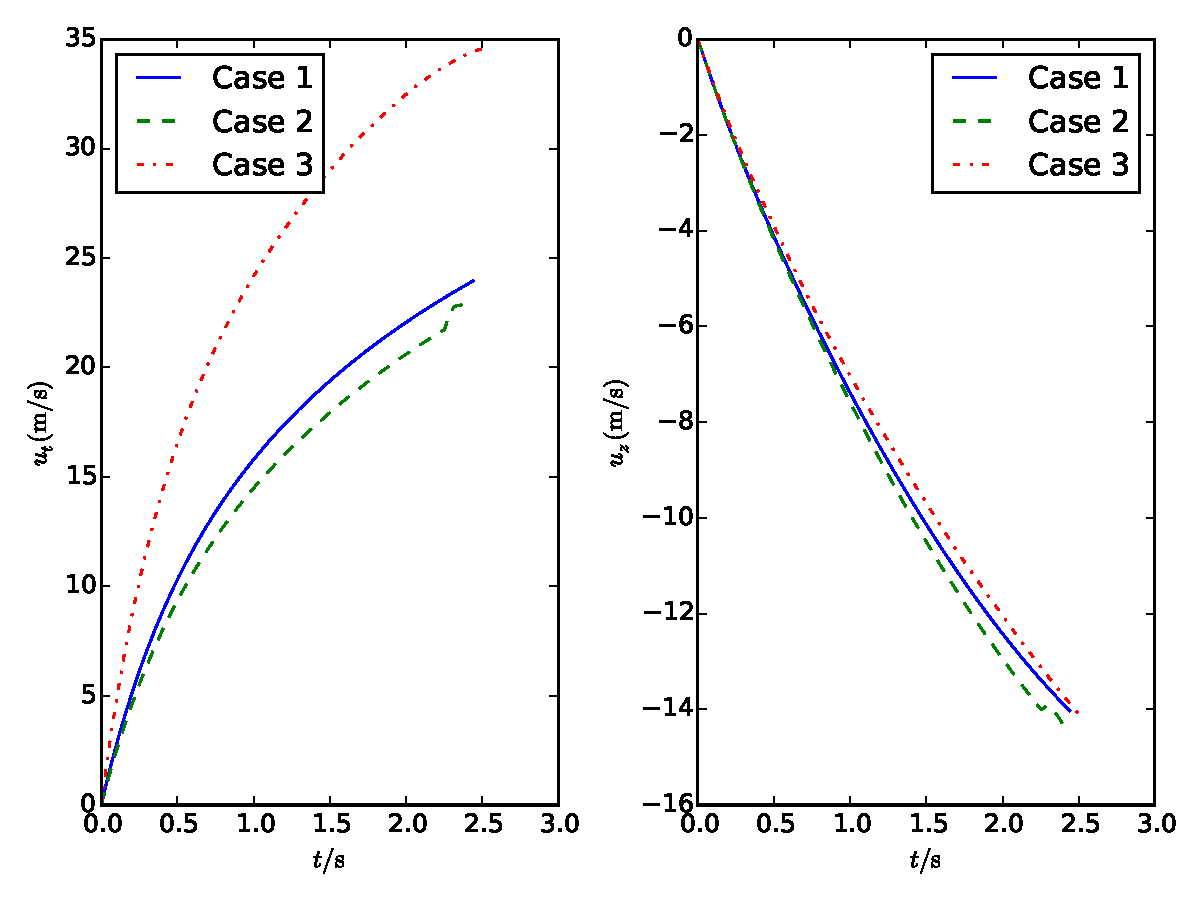
\includegraphics[width=0.8\linewidth]{./calculation/velocity_history}
\caption{圆球飞行过程中切向速度和竖向速度的时程曲线(Case 1, 2, 3)}
\label{fig:velocity_history}
\end{figure}

可以看出,三种计算方法中,Case 1和Case 2误差较小,互相验证了小时间部积分法与ANSYS Fluent软件求解方法在计算Rankine涡中飞射物的运动的正确性。
Case 3的计算方法采用直接模拟龙卷风的方法,根据第\ref{sec:cfd_verification}中的讨论,直接模拟的龙卷风风场与Rankine涡存在不同,引起该算例中圆球切向速度明显大于Case 1和Case 2的原因如下:
\begin{itemize}
  \item 直接模拟的龙卷风风场,半径$r=\SI{300}{m}$处风场切向速度大概为$V_r=\SI{38.30}{m/s}$(见图\ref{fig:Vr});而按照Rankine涡模型,半径$r=\SI{300}{m}$处风场切向速度为$V_r=\frac{\mathrm{R}}{r}V_{\mathrm{R}}=\SI{32.26}{m/s}$。
  \item
  直接模拟的龙卷风风场存在径向速度,会引起圆球向涡旋中心运动,而在此算例中,此径向运动会使得飞射物所在的流场处的切向风速增大。算例中,圆球的初始径向位置$r_0=\SI{300}{m}$,落地时的径向位置为$r=\SI{281.55}{m}$,龙卷风的切向速度由大概$\SI{38.30}{m/s}$增大到大概$\SI{41.65}{m/s}$。
  \item
  直接模拟的龙卷风风场存在竖向速度,会使得圆球下落的加速度减小,会延长圆球的飞行时间,但据表\ref{tab:compact}可以看出,这一影响较小,可忽略不计。
\end{itemize}

为了直观上观察上述因素的影响,再引入以下计算情形:
\begin{description}
\item[Case 4: ] 采用《龙卷风风场中块状飞射物的飞行特性:解析方法》中考虑竖向速度对风阻力影响的小时间步积分法计算飞射物的运动过程,将风场切向速度取为$\SI{38.30}{m/s}$,以考虑直接模拟的龙卷风风场的切向速度大于Rankine涡模型的影响。
\item[Case 5: ] 采用《龙卷风风场中块状飞射物的飞行特性:解析方法》中考虑竖向速度对风阻力影响的小时间步积分法计算飞射物的运动过程,将风场切向速度取为$\SI{41.65}{m/s}$,以考虑圆球径向运动到切向速度较大的位置。
\end{description}
Case 3、4和5的情形下,圆球的运动情况如图\ref{fig:velocity_history2}所示。
\begin{figure}
\centering
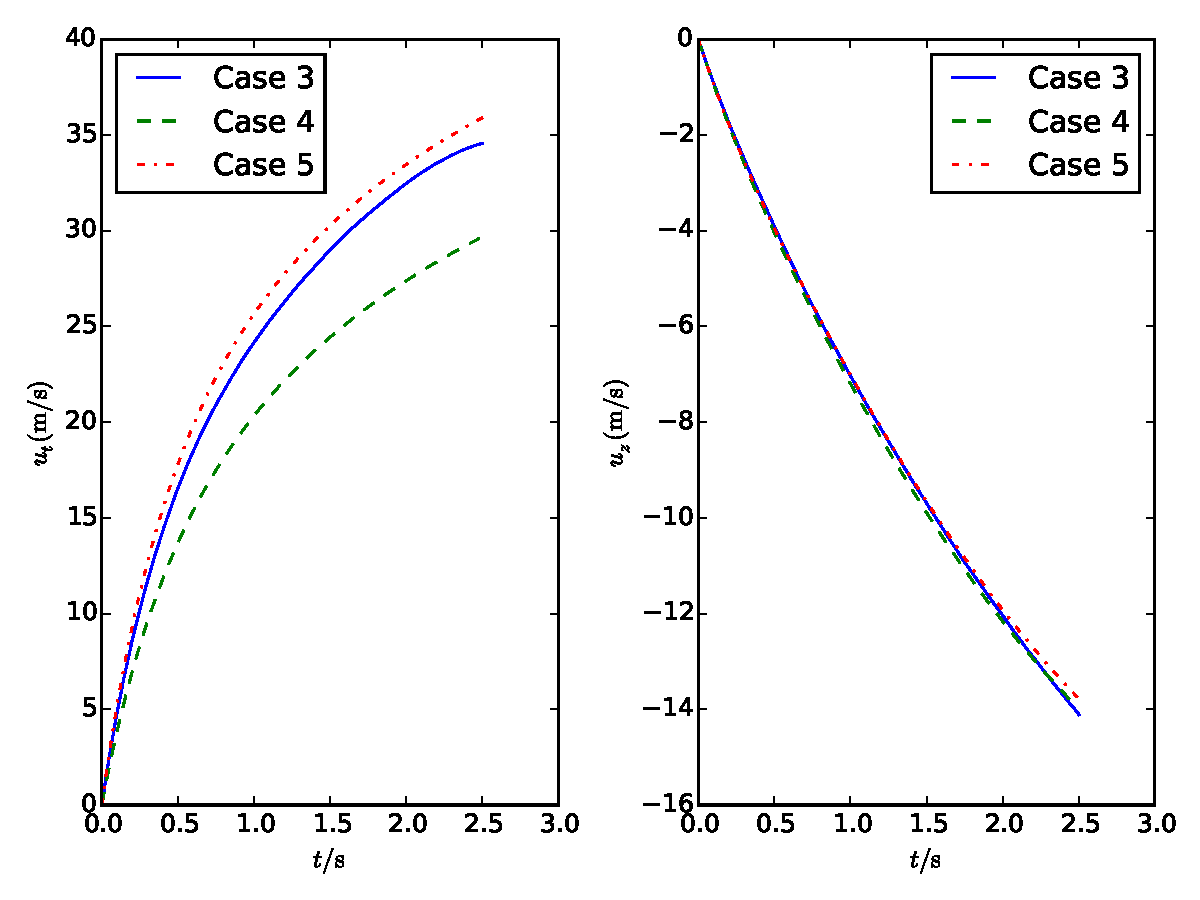
\includegraphics[width=0.8\linewidth]{./calculation/velocity_history2}
\caption{圆球飞行过程中切向速度和竖向速度的时程曲线(Case 3, 4, 5)}
\label{fig:velocity_history2}
\end{figure}
可见,根据直接模拟的龙卷风风场和圆球径向运动的情况,调整Rankine涡模型中的切向速度,利用小时间步积分方法可以逼近圆球在直接模拟龙卷风风场中的运动。
\newpage
\printbibliography
\end{document}